\chapter{Grundlagen und Forschungsstand}

Neben einer Einführung in den Anwendungsbereich von \textit{Deep Learning} zur Bildverarbeitung soll sich das folgende Kapitel speziell mit Architekturen unterschiedlicher Objektdetektoren auseinander setzen und herausstellen, wie sich diese voneinander abgrenzen. Davor wird allerdings zunächst grundlegendes Wissen über neuronale Netze und wie diese \glqq lernen\grqq{} vermittelt sowie über Hyperparameter und wie ein eigener Datensatz zu gestalten ist.

\section{Deep Learning zur Bildverarbeitung} \label{bildverarbeitung}

Ein klassisches Anwendungsgebiet von \textit{Deep Learning} zu Bildverarbeitung oder auch allgemein von maschinellem Lernen beschreibt die \textit{Klassifikation}. Hierbei werden bestimmte Kategorien, auch \textit{Klassen} genannt, definiert, in die ein Bild eingeordnet werden soll. Die \textit{Klassifikation} wird anhand von aus dem Bild extrahierten Merkmalen, auch \textit{Features} genannt, getroffen. Die Merkmale werden zu einem \textit{Merkmalsvektor} oder auch \textit{Feature Map} zusammengefasst und von einem \textit{neuronalen Netz} verarbeitet. Das Ergebnis der Verarbeitung durch das neuronale Netz ist die Einordnung in eine bestimme Klasse. 

Zusätzlich zur \textit{Klassifikation} eines Bildes kann das auf dem Bild abgebildete Objekt ebenfalls lokalisiert werden. Es wird dann von sogenannter \textit{Objektdetektion} gesprochen. Es können auch mehrere Objekte auf einem Bild detektiert werden. Ergebnis der Objektdetektion ist somit nicht nur eine Klasseneinordnung sondern ebenso eine klare Positionsangabe des Objektes auf dem Bild. Die Positionsangabe erfolgt durch Angabe einer sogenannten \textit{Bounding Box}. Diese umrahmt das jeweils detektierte Objekt und wird durch ihren linken oberen Eckpunkt sowie ihre Höhe und Breite beschrieben. 

Neben der klassischen \textit{Klassifikation} und der \textit{Objektdetektion} existiert ebenso ein drittes Anwendungsgebiet von \textit{Deep Learning} zu Bildverarbeitung, die \textit{Segmentierung}. Bei der \textit{semantischen Segmentierung} wird versucht, jede einzelne Pixel eines Bildes einer Klasse zuzuordnen und dementsprechend farblich im Bild zu hinterlegen. \textit{Instanzbasierte Segmentierung} hingegen zielt darauf ab, nicht nur jeden Pixel zu einer Klasse zuzuordnen, sondern ebenso eine Identität zu einem Objekt zuzuweisen. Es setzt sich zusammen aus \textit{semantischer Segmentierung} und paralleler \textit{Objektdetektion} \cite{AlexKrizhevskyIlyaSutskeverGeoffreyE.Hinton.2012,RossGirshickJeffDonahueTrevorDarrellJitendraMalik.2016,FarhanaSultanaAbuSufianParamarthaDutta.20200210}.

Einen Überblick über die vorgestellten Anwendungsgebiete ist in Abbildung \ref{applications} zu sehen.

\begin{figure}[H]
	\begin{center}
		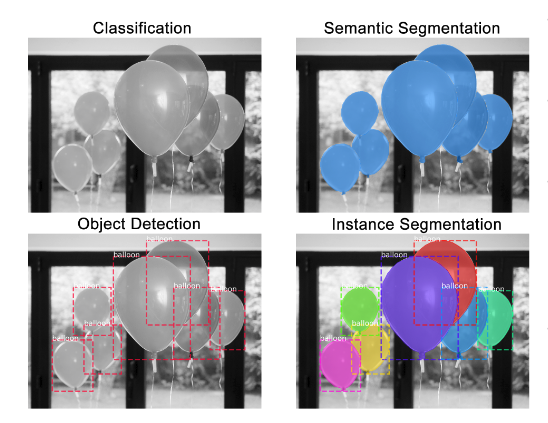
\includegraphics[width=12cm]{Bilder/applications.png} 
		\caption[Anwendungsgebiete von Deep Learning zur Bildverarbeitung im Überblick]{Anwendungsgebiete von Deep Learning zur Bildverarbeitung im Überblick \cite{PriyaDwivedi.20190328}}
		\label{applications}
	\end{center}
\end{figure}

Für eine einfache \textit{Klassifikation} eines Bildes können einfache sogenannte \textit{Feed-Forward} Netze verwendet werden. Es kann hierbei aber auch auf konventionelle Methoden der Bildverarbeitung zurück gegriffen werden. Für die \textit{Objektdetektion} stehen Architekturen wie \textit{You Only Loom Once} (YOLO), der \textit{Single Shot MultiBox Detector} (SSD) oder neuronale Netze der \textit{Regional Convolutional Neural Networks} (R-CNN) bereit. Aus dieser Familie entstammt ebenso das \textit{Mask R-CNN} Netz, das zur \textit{instanzbasierten Segmentierung} von Objekten verwendet wird.
